\documentclass[]{beamer}
\usepackage{tbagrelbeamer}
\usepackage{beamerstylebluesky}
\usepackage{pgfplots}

\begin{document}

\title{Deep learning}
\subtitle{CNN and supervised learning}
\author{March 2019 @ TELECOM Nancy\\T. \sc{Bagrel}}
\date{}

\begin{frame}
  \titlepage{}
\end{frame}

% \begin{frame}
%   \frametitle{}
%   \framesubtitle{}
% \end{frame}

\begin{frame}
  \frametitle{Introduction}
  \framesubtitle{Interesting NN architectures (supervised)}
  \begin{block}{\bf{C}onvolutional \bf{N}eural \bf{N}etwork (CNN)}
    \begin{itemize}
      \item \alert{Supervised \tt{:(}}
      \item Most common architecture for image processing
      \item Position-invariant feature extraction (with shared weights)
      \item Very efficient
    \end{itemize}
  \end{block}
\end{frame}
\begin{frame}
  \frametitle{Introduction}
  \framesubtitle{Interesting NN architectures (unsupervised)}
  \begin{block}{\bf{R}estricted \bf{B}oltzmann \bf{M}achine (RBM)}
    \begin{itemize}
      \item \alert{Unsupervised!}
      \item General feature extraction
      \item Basic block of \bf{D}eep \bf{B}elief \bf{N}etworks
    \end{itemize}
  \end{block}
  \begin{block}{\bf{A}uto\bf{e}ncoders (AE)}
    \begin{itemize}
      \item \alert{Unsupervised!}
      \item Can be used for denoising
      \item Can be used for general feature extraction
    \end{itemize}
  \end{block}
\end{frame}

\begin{frame}
  \frametitle{Autoencoders}
  \framesubtitle{Structure and principle}
  \begin{block}{Principle}
    \begin{itemize}
      \item \alert{Simple} : reproduce the input at the output
      \item \alert{How} : pass the input (image) through the NN, compute error from $\text{diff}(I, O)$, adjust weights with GD
    \end{itemize}
  \end{block}
  \begin{exampleblock}{Feature extraction}
    \alert{Bottleneck} : ``center'' of the NN where there is the lowest number of neurons. Activation in the ``bottleneck'' for a given input (image) represents its compressed form.
  \end{exampleblock}
\end{frame}

\begin{frame}
  \frametitle{Autoencoders}
  \framesubtitle{Denoising}
  \begin{center}
    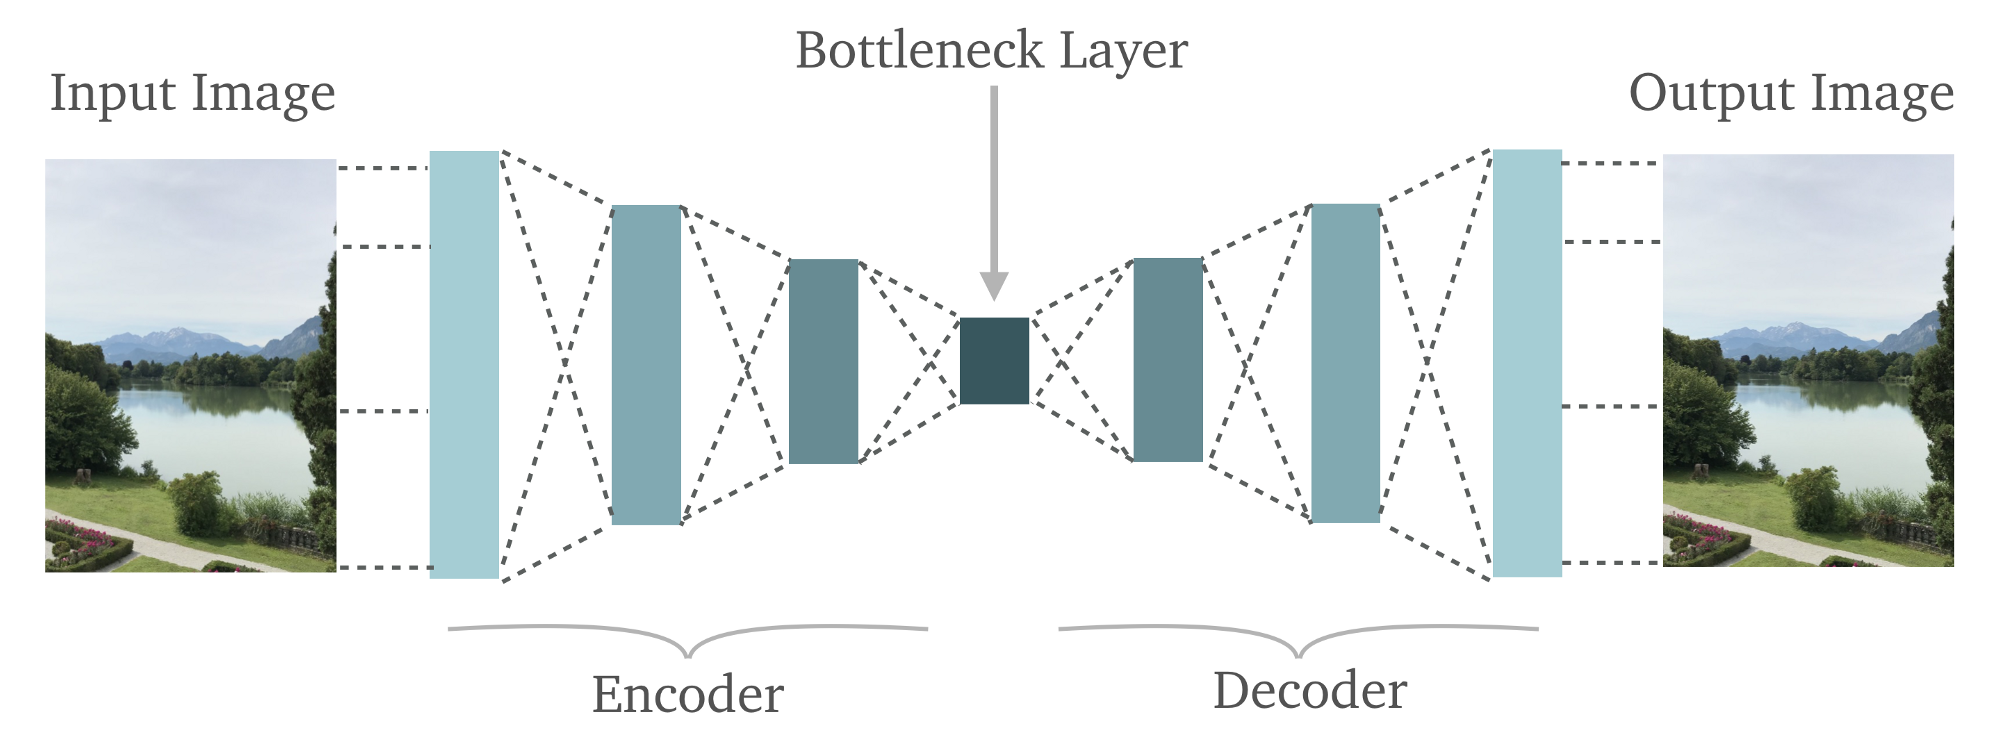
\includegraphics[width=\linewidth]{resources/autoencoder}
    \captionof{figure}{Autoencoder with feature extraction purpose}
  \end{center}

  \begin{exampleblock}{Denoising}
    Denoising can be achieved with roughly the same architecture
  \end{exampleblock}

\end{frame}

\begin{frame}
  \frametitle{CNN Components}
  \framesubtitle{Gradient Descent}
  \begin{center}
    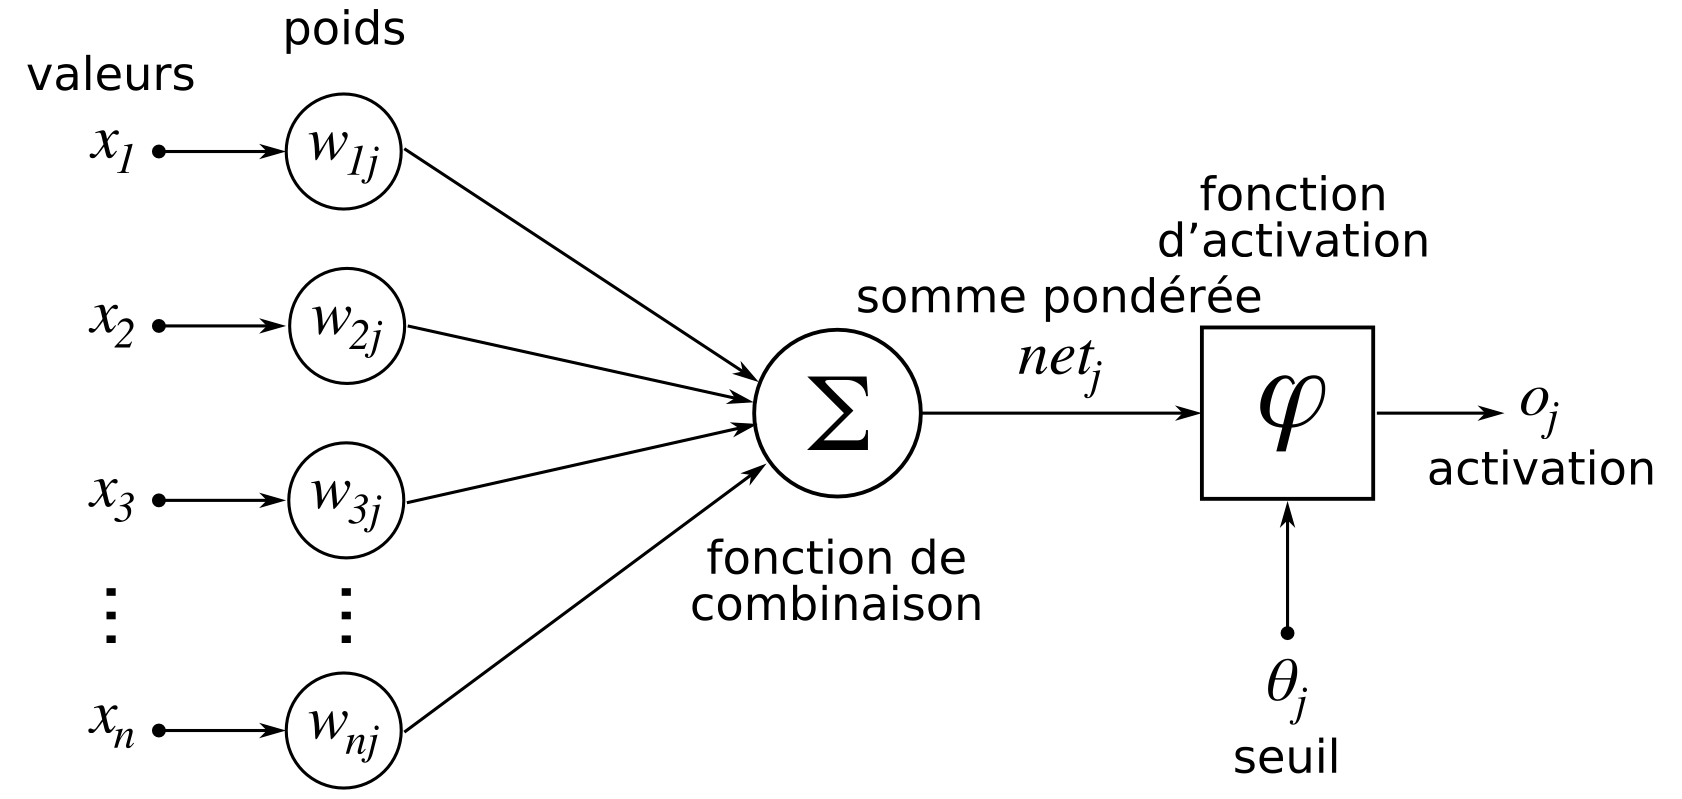
\includegraphics[width=\linewidth]{resources/perceptron}
    \captionof{figure}{Neuron (perceptron) schema}
  \end{center}
\end{frame}

\begin{frame}
  \frametitle{CNN Components}
  \framesubtitle{Gradient Descent}
  \begin{block}{Problem solved by GD}
    In which direction do we need to update our weights to minimize the error?
  \end{block}
  \begin{exampleblock}{Last layer neuron $n$ situation}
    $E$: error, $L$: loss function, $e$: expected value, $o$: obtained value, $\phi$: activation function, $x_{n, \cdot}$: inputs for the last layer neuron, $w_{n, \cdot}$: weights for the last layer neuron
    \begin{IEEEeqnarray}{rCl}
      E &=& L(e, o) \\
        &=& L\left(e,~~~\phi\left(\sum_k x_{n, k} w_{n, k}\right)\right)
    \end{IEEEeqnarray}
  \end{exampleblock}
\end{frame}

\begin{frame}
  \frametitle{CNN Components}
  \framesubtitle{Gradient Descent}
  \begin{exampleblock}{What we need to know}
    \begin{itemize}
      \item \alert{loss function} $L(e, o)$ and $\dfrac{\partial{}L}{\partial{o}}$
      \item \alert{activation function} $\phi(r)$ and $\dfrac{\mrm{d}\phi}{\mrm{d}r}$
    \end{itemize}
  \end{exampleblock}
  \begin{exampleblock}{What we can compute}
    With the \alert{chain rule}, we can compute $\dfrac{\partial{}E}{\partial{}w_{n, k}}(e, o) \quad (\forall k)$
  \end{exampleblock}
\end{frame}

\begin{frame}
  \frametitle{CNN Components}
  \framesubtitle{Gradient descent and adjustment made}
  \begin{block}{Weights adjustment ($\alpha$ : learning rate)}
    \[ w_{n, k} \longleftarrow w_{n, k} - \alpha \cdot \dfrac{\partial{}E}{\partial{}w_{n, k}}(e, o) \]
  \end{block}
  \begin{center}
    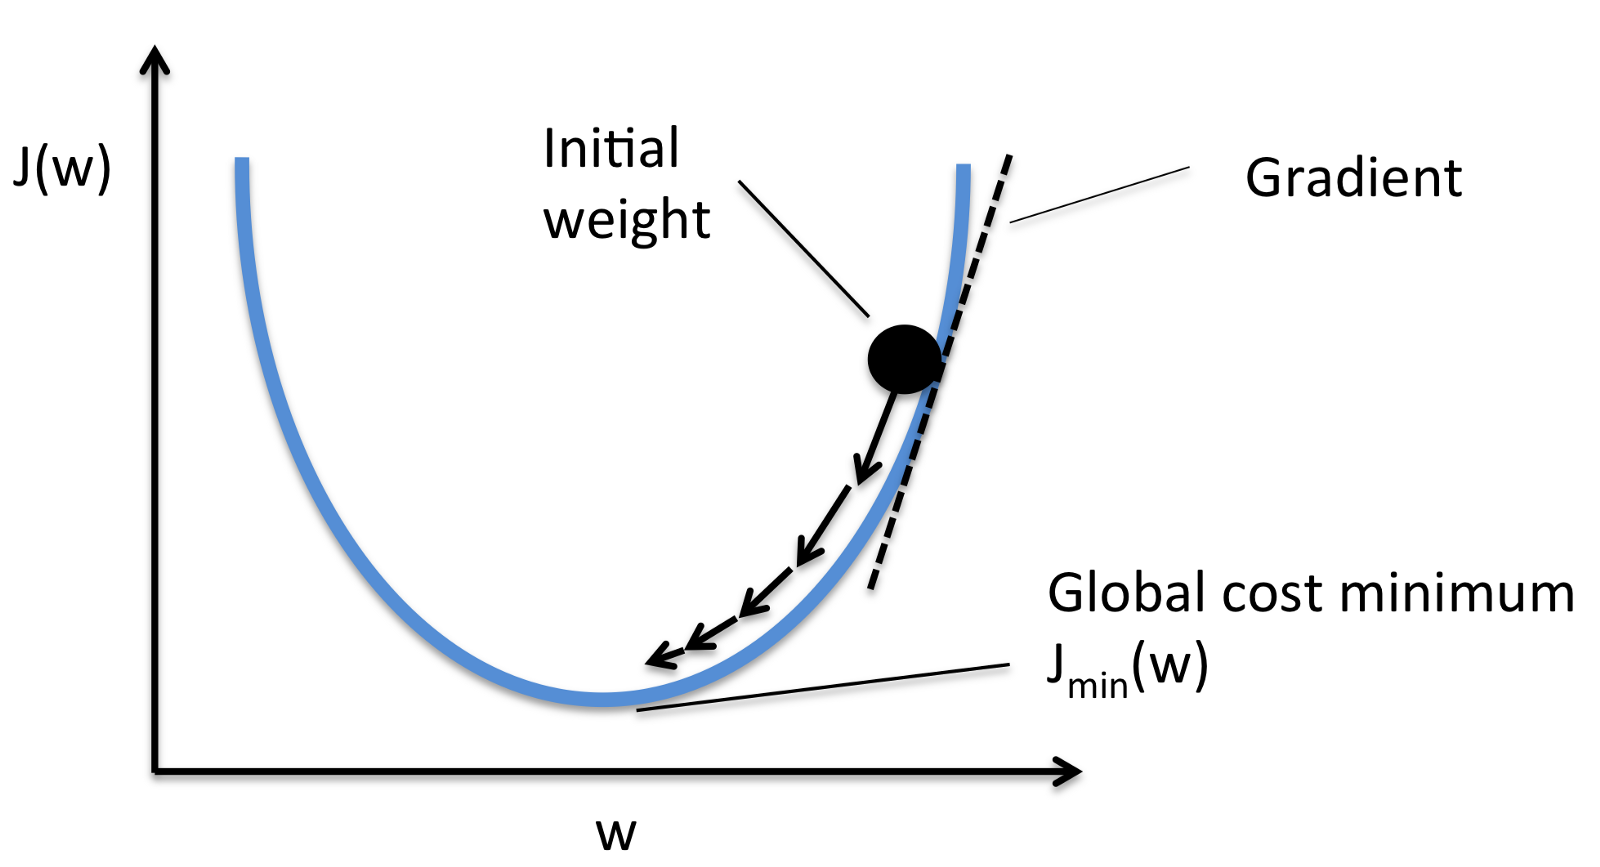
\includegraphics[width=0.8\linewidth]{resources/gd}
  \end{center}
\end{frame}

\begin{frame}
  \frametitle{CNN Components}
  \framesubtitle{Learning rate and advanced adjustment methods}
  \begin{center}
    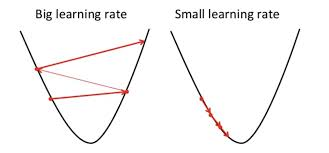
\includegraphics[width=\linewidth]{resources/big_vs_small_lr}
    \captionof{figure}{Importance of an appropriate learning rate}
  \end{center}
\end{frame}

\begin{frame}
  \frametitle{CNN Components}
  \framesubtitle{Advanced adjustment methods}
  Called optimizers in \alert{TensorFlow}
  \begin{block}{Roles}
    \begin{itemize}
      \item Try to prevent staying in a non-global local minima during learning
      \item \alert{Examples} : Nesterov Momentum, Adam\ldots{}
    \end{itemize}
  \end{block}

  \begin{exampleblock}{Used in my NNs}
    I use Nesterov's momentum: \tt{optimizers.SGD(nesterov=True, momentum=M)}\\ because it's recommended on most tutorials
  \end{exampleblock}
\end{frame}

\begin{frame}
  \frametitle{CNN Components}
  \framesubtitle{GD vs SGD vs BGD}
  Each one is a different manner to apply Gradient Descent
  \begin{block}{Differences}
    \begin{itemize}
      \item \alert{(basic) Gradient Descent} : weights are updated after every epoch (whole dataset pass) $\to$ \alert{very costly} but more stable than SGD!
      \item \alert{Stochastic Gradient Descent} : weights are updated after \alert{every} sample $\to$ \alert{very fast}!
      \item \alert{Batch Gradient Descent} : weights are updated after $N$ samples ($10 \le N \le 100$: batch size) $\to$ \alert{best of both worlds!}
    \end{itemize}
  \end{block}
\end{frame}

\begin{frame}
  \frametitle{CNN Components}
  \framesubtitle{Convolutional layer}
  The (3D) \alert{dot product} between the \alert{filter weights} and an \alert{input image zone} of the same size/shape gives an activation value. Doing this operation for all possible image zones (with \bf{overlap}) gives the \alert{activation map} for this filter.

  \it{It explains the position invariance of feature extraction for CNNs!}
  \begin{center}
    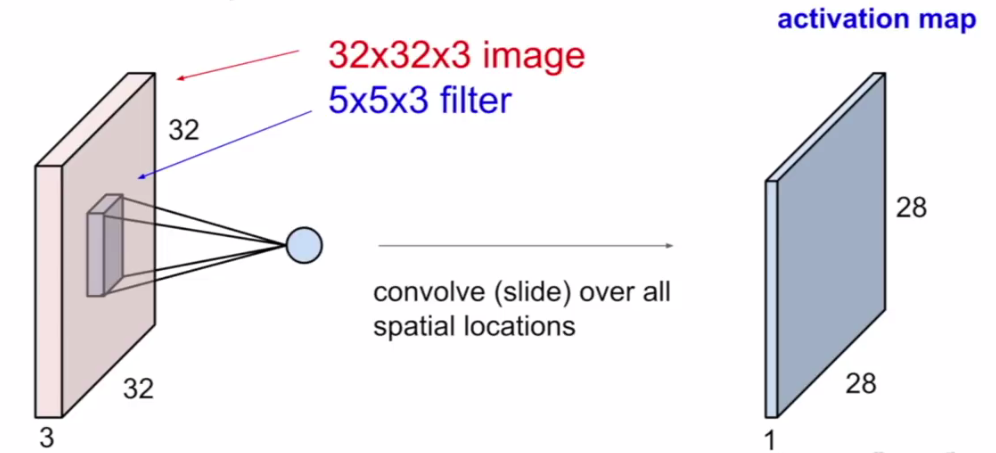
\includegraphics[width=0.8\linewidth]{resources/conv_1}
  \end{center}
\end{frame}

\begin{frame}
  \frametitle{CNN Components}
  \framesubtitle{Convolutional layer}
  A \alert{convolutional layer} is composed of several filters, each one with its \alert{own weights}. Hence, the output of the convolutional layer is a \alert{stack of activation maps} (one for each filter)
  \begin{center}
    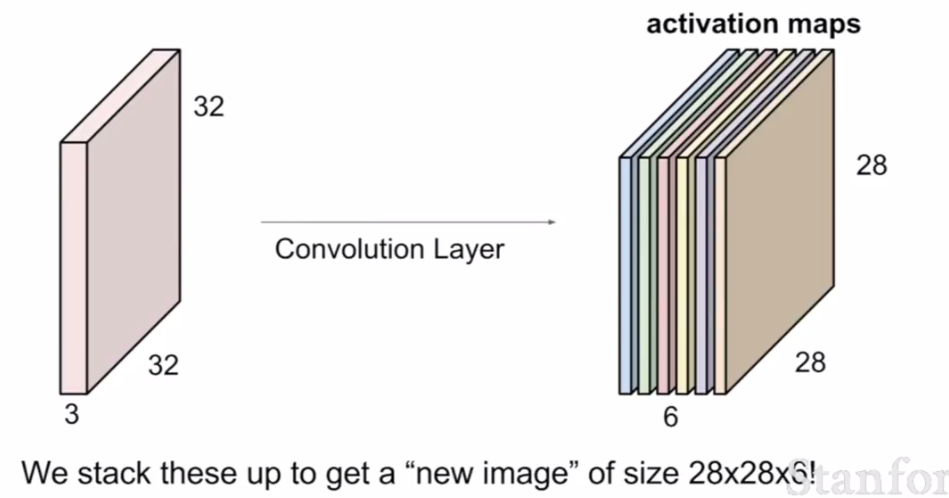
\includegraphics[width=0.8\linewidth]{resources/conv_2}
  \end{center}
\end{frame}

\begin{frame}
  \frametitle{CNN Components}
  \framesubtitle{Pooling layer}
  A \alert{pooling layer} is used to downsize/down-sample its input. \alert{All} the values in a zone of the input volume results in \alert{one} value in the output volume, by application of a simple function. Input zones \bf{must not overlap} here!

  A very common example is the \it{max pooling} 2 x 2:
  \begin{center}
    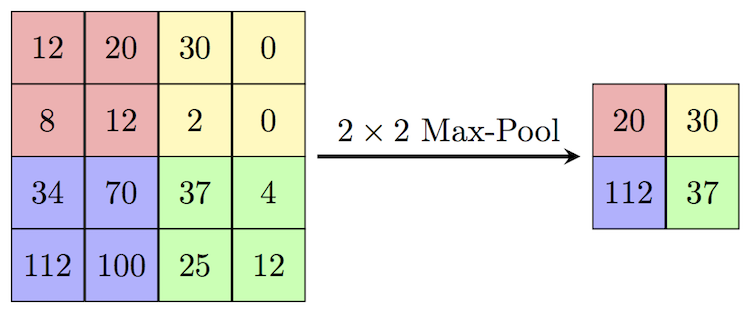
\includegraphics[width=\linewidth]{resources/pool}
  \end{center}
\end{frame}

\begin{frame}
  \frametitle{CNN Components}
  \framesubtitle{Output layer for classification}
  The output layer is used to extract classification information from a final dense/convolutional/pooling layer.
  \begin{block}{Types}
    \begin{itemize}
      \item For binary classification: Dense layer with \alert{sigmoid} activation function and \alert{1} neuron (1 output value)
      \item For multiclass classification : Dense layer with \alert{softmax} activation function and \alert{$\text{Nb}_{\text{classes}}$} neurons, followed by a $\text{arg\_max}(\cdot\cdot\cdot)$ function
    \end{itemize}
  \end{block}
\end{frame}

\begin{frame}
  \frametitle{CNN Components}
  \framesubtitle{Loss function for classification}
  \alert{Cross entropy} (aka. Negative Log Likelihood) is the loss function used in classification, which works well with the \alert{sigmoid} or \alert{softmax} activation functions (output layer)
  \begin{center}
    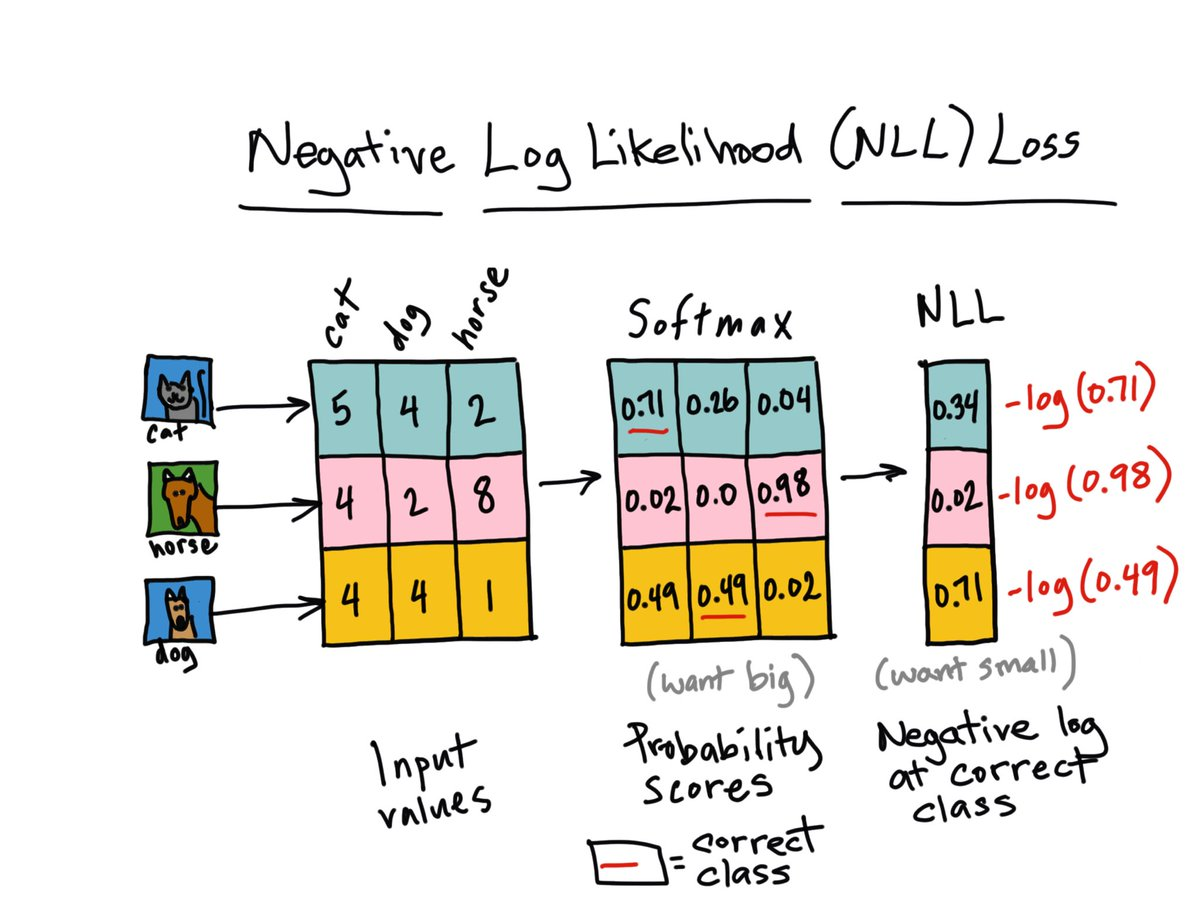
\includegraphics[width=0.7\linewidth]{resources/nll}
  \end{center}
\end{frame}

% medical images
% why not ?
% creation
% brain_tumor
% base image
% C program
% image generation
% alter
% types
% easy / hard
% guess it
% what can be achieved
% overfitting
% regularization
% underfitting
% evolutions of the nn

% hardware & software
% dl4j
% cpu vs gpu
% tensorflow
% futur equipment ?

% credits

\end{document}
